\documentclass{article}%
\usepackage[T1]{fontenc}%
\usepackage[utf8]{inputenc}%
\usepackage{lmodern}%
\usepackage{textcomp}%
\usepackage{lastpage}%
\usepackage{authblk}%
\usepackage{graphicx}%
%
\title{Regulation of Histone Acetylation in the Nucleus by Sphingosine{-}1{-}Phosphate}%
\author{Shane Macias}%
\affil{Institute of Pharmacology, Toxicology and Pharmacy, Ludwig{-}Maximilians{-}University, Munich, Germany}%
\date{01{-}01{-}2008}%
%
\begin{document}%
\normalsize%
\maketitle%
\section{Abstract}%
\label{sec:Abstract}%
As youre brushing your teeth for the first time, prepare to take a second peek under the rim to see the markers that are all over your mouth.\newline%
Whatever the case, a new study has discovered a protein that is present in nasties is also present in healthy tissue, and appears to be enhancing the restoration of the tissues to a more normal state.\newline%
Isabell Maynard developed a protein using an ultra{-}high{-}tech process called stem cell transplantation. She transplanted a 5 year old girls stem cells into the patients right leg and found that the two tissue classes were getting more and more liquid, complementing each other in what may be a first{-}of{-}its{-}kind approach for a patients fibrous tissue to benefit from a simple clearing.\newline%
Maynard said, And these little guys that are there now are being flush with their protective building blocks which gives them super strength and I think for the first time in medicine it really does confer some kind of health benefit.\newline%
During development the new{-}found protein that Maynard engineered and transplanted into the patients leg was swollen up, but when placed through a series of tubes, gradually became lighter and more elastic, allowing each other to breathe.\newline%
Maynard continues, And I think it would make an incredible difference if we could start to roll back the damage from ultraviolet radiation and exposure to all of these pollutants and our poor energy consumption patterns.\newline%
Maynard said a transplant is an option for young children, but if this helps lower symptoms and even preventing some diseases, it could offer the option of long{-}term clinical benefits of multiple sclerosis and bone cancer.\newline%
A paper describing the mouse experiments was recently published in the journal Nature.

%
\subsection{Image Analysis}%
\label{subsec:ImageAnalysis}%


\begin{figure}[h!]%
\centering%
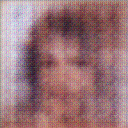
\includegraphics[width=150px]{500_fake_images/samples_5_433.png}%
\caption{A Black And White Photo Of A Black And White Cat}%
\end{figure}

%
\end{document}